% TEMPLATE for Usenix papers, specifically to meet requirements of
%  USENIX '05
% originally a template for producing IEEE-format articles using LaTeX.
%   written by Matthew Ward, CS Department, Worcester Polytechnic Institute.
% adapted by David Beazley for his excellent SWIG paper in Proceedings,
%   Tcl 96
% turned into a smartass generic template by De Clarke, with thanks to
%   both the above pioneers
% use at your own risk.  Complaints to /dev/null.
% make it two column with no page numbering, default is 10 point

% Munged by Fred Douglis &lt;douglis@research.att.com&gt; 10/97 to separate
% the .sty file from the LaTeX source template, so that people can
% more easily include the .sty file into an existing document.  Also
% changed to more closely follow the style guidelines as represented
% by the Word sample file. 

% Note that since 2010, USENIX does not require endnotes. If you want
% foot of page notes, don't include the endnotes package in the 
% usepackage command, below.

% This version uses the latex2e styles, not the very ancient 2.09 stuff.
\documentclass[letterpaper,twocolumn,10pt]{article}
\usepackage{usenix,epsfig,endnotes}
\usepackage{kotex}
\usepackage{subfigure}
\usepackage{comment}
\begin{document}

%don't want date printed
\date{}

%make title bold and 14 pt font (Latex default is non-bold, 16 pt)
\title{\Large \bf Unified Storage Layer: Eliminating the Compound
Garbage Collection in Log-Structured Filesystem for Flash Storage}

%for single author (just remove % characters)
%\author{
%{\rm Your N.\ Here}\\
%Your Institution
%\and
%{\rm Second Name}\\
%Second Institution
% copy the following lines to add more authors
% \and
% {\rm Name}\\
%Name Institution
%} % end author

\maketitle

% Use the following at camera-ready time to suppress page numbers.
% Comment it out when you first submit the paper for review.
\thispagestyle{empty}


\subsection*{Abstract}
Log-structured system은 데이터를 append 방식으로 기록하므로 sequential 쓰기의 특성을 보이며, 시스템 crach 상황 시 복구에도 용이하다. 그러나 데이터 업데이트로 인해 발생한 무효화(Invalidation)된 데이터를 제거하여 시스템 공간을 확보하는 가비지 컬렉션 동작이 필요하며, 이는 로그 기반 시스템의 성능 저하 요인으로 작용한다. 더욱이 로그 기반 시스템 계층이 2개 이상 중첩되면 메타데이터 관리 overhead가 증가하고, 각 계층에서 모두 가비지 컬렉션 동작을 수행하므로, 하단의 디바이스 계층이 받는 입출력 부하가 더욱 증폭되게 된다. 이를 Compound Garbage Collection 문제라 한다. 우리는 이러한 중첩된 로그 시스템에서의 문제를 해결하기 위하여 Unified Storage Layer 기법을 제안한다. Unified Storage Layer는 파일시스템과 SSD 펌웨어가 서로를 인지하여 동작하도록 하여 불필요한 동작을 제거하고 관리에 필요한 메타데이터 크기를 줄이는 최적화 기법을 사용한다. 로그 방식 파일시스템인 F2FS의 각 영역 특성에 적합한 매핑 scheme을 사용하는 disaggregate mapping 기법을 개발하여 SSD 펌웨어에 적용하였으며, 이를 통해 SSD 메타데이터의 크기를 기존 대비 54분의 1로 감소시켰다. 사용자 데이터 영역에 대해서는 파일시스템에서 통합하여 가비지 컬렉션 동작을 수행하게 하고, 이에 해당하는 SSD 영역의 가비지 컬렉션 동작을 제거함으로써 Compound Garbage Collection 문제를 해결하였다. 이와 같은 기법을 적용한 Unified Storage Layer는, 기존 중첩된 로그 시스템의 쓰기 증폭을 40\% 감소 시킴과 동시에 77\% 높은 IOPS를 보였으며, SSD의 메타데이터 관리에 필요한 메모리의 사이즈를 크게 줄일 수 있었다.


\section{Introduction}

플래시 메모리를 저장매체로 사용하는 Solid State Drive(SSD)는 기존의 Hard Disk Drive(HDD) 대비 짧은 입출력 지연, 적은 전력 소모, 높은 충격저항을 장점으로 갖는 스토리지이다. 그러나 In-place update가 되지 않는 플래시 메모리 소자의 특성으로 인해, 이미 스토리지에 저장된 데이터를 update하는 write operation을 수행하기 전에, write operation 보다 수 배의 지연시간을 갖는 erase operation이 선행되어야 한다. 더욱이 erase operation은 SSD의 쓰기 단위인 페이지(e.g. 4$\sim$16KByte) 보다 큰, 수 Mbyte 크기의 블록 단위로 수행되며 이는 SSD의 성능 저하 요인으로 작용한다. SSD의 이러한 문제점을 해결하기 위하여, 쓰기 요청을 out-of-place 방식으로 처리하기 위한 소프트웨어 계층인 Flash Translation Layer(FTL)가 SSD 펌웨어에 탑재되어 동작한다. FTL은 매 쓰기 요청을 SSD의 빈 페이지에 기록함으로써 SSD erase opeation의 지연시간을 Host로 부터 감추도록 한다. 즉, 호스트로부터 동일한 LBA에 대한 쓰기 요청을 전달 받더라도, SSD 상에서 기록되는 물리 페이지의 위치는 계속하여 변경되게 된다. 이러한 동작을 지원하기 위해 Host가 전달한 주소(Logical Block Address)와 실제 SSD에 데이터가 위치한 주소(Physical Block Address)를 매칭하는 매핑 테이블을 관리한다. FTL은 Host가 SSD를 기존의 블록 디바이스와 동일한 인터페이스를 사용하여 호스트와 동작할 수 있도록 하는 Abstraction Layer로서 기능한다. 

그러나 이러한 FTL의 Logical to Physical 매핑은 입출력 stack의 복잡도를 증가시키며, 크게는 가비지 컬렉션 동작과 메타데이터 관리 overhead를 야기한다. 매번 새로운 페이지에 쓰기 요청을 수용하는 FTL의 정책은, SSD 내에 무효한 데이터들을 쌓이게 한다. For example, when a data is updated, then the data in the original location is invalidated and new version of the data is appended at the end of the log-structured filesystem. As the number of invalid data increases, garbage collection is inevitable and crucial operation to maintain the system. 가비지 컬렉션 동작은 호스트의 입출력 요청과는 별개로 SSD 내부적으로 발생하여 수행되는 동작이므로, SSD의 성능 저하 요인으로 작용한다. 또한, 매핑 정보 자체의 크기만으로도 SSD의 overhead가 된다. SSD의 페이지 단위로 매핑 정보를 관리하는 페이지 매핑 방식의 경우, 8Kbyte 크기의 페이지를 갖는 256GByte 용량의 SSD의 경우 128MByte 크기의 매핑 정보를 관리해야 한다. 매핑 정보는 SSD 내부의 SRAM 또는 DRAM에 로드 되어 정보를 갱신하게 되므로, 매핑 정보의 크기가 클 수록 더 큰 DRAM을 요구하게 된다. 이러한 문제는 SSD의 크기가 대용량화 됨에 따라 더욱 심각해 지는데, 이를 테면 4TByte의 SSD를 관리하기 위해서는 2GByte 크기의 매핑 정보가 필요하게 된다.

이와 같이 파일시스템 - 블록 I/O 계층 - 디바이스 드라이버 - FTL로 이어지는 IO 계층 구조는, 호스트가 플래시 메모리의 성능을 충분히 활용할 수 없도록 한다. 이러한 문제점을 해결하기 위하여 Fusion IO\cite{fusion_io}는 FTL의 기능을 디바이스 드라이버 계층으로 옮기어, 파일시스템이 플래시 메모리 기반 저장장치의 layout을 알 수 있도록 하였으며, 디바이스 드라이버에서 블록 할당, 가비지 컬렉션, 매핑 정보 등의 관리를 수행하도록 한다. 이러한 구현 방식은 파일시스템의 구현을 간단하게 할 수 있도록 하며, 호스트 레벨에서 FTL 동작을 처리하므로 호스트의 CPU, 메모리와 같은 자원을 활용할 수 있도록 한다. 그러나 FusionIO의 이러한 방식 또한 매핑 정보의 크기 overhead에서 자유롭지 못하며, 더욱이 PCIe 기반의 자체 저장장치인 FusionIO에서만 동작할 수 있는 한계를 갖는다.

SSD의 성능을 활용하기 위한 노력은 파일시스템에서도 진행되어 왔다. Flash-Friendly File System(F2FS\cite{lee2015f2fs})은 플래시 메모리 기반 저장장치를 타겟으로 하는 로그 기반의 파일시스템이다. Since Log structured systems\cite{rosenblum1992design} perform all writes in append-only style, its workload pattern has sequential write characteristics, which increases the performance of write operations. However, it comes with serious cost of garbage collection. 이러한 이유로 기존의 로그 기반 파일시스템들은 In-place update 방식의 파일시스템(E.g. Ext4\cite{cao2007ext4})에 비해 낮은 입출력 성능을 보였다\cite{jeong2013stack}. 그러나 F2FS의 경우 플래시 메모리의 동작을 염두한 블록 할당 정책, 가비지 컬렉션 정책 등으로 Ext4 대비 특정 워크로드에서 크게는 3.1배 높은 입출력 성능을 보인다\cite{lee2015f2fs}. F2FS의 등장은 플래시 기반 스토리지에서 로그 기반 파일시스템의 사용을 재 조명하도록 하였다.

그러나 한편에서는 로그 기반 파일시스템을 플래시 기반 스토리지에서 사용하는 것의 문제점을 지적한다. Yang et al\cite{yang2014don}은 그 연구에서 플래시 기반 스토리지에 로그 기반 파일시스템의 쓰기 방식이 적합함을 언급하면서도, FTL, 로그 기반 파일시스템, 로그 기반 DB 등이 적층되어 'Log stacking model'을 구성하였을 때의 문제점을 제시한다. 첫 번째로, 각 로그 시스템은 새로운 위치에 데이터를 기록하기 위한 매핑 정보를 유지해야 하며, 각 로그 시스템마다 유지해야되는 이러한 매핑 정보는 메타 데이터 관리 overhead를 증가시킨다. 두 번째로, When append only log-structured filesystem meets out-of-place only storage device, that is SSD, they create interesting yet severe problem called compound garbage collection; when two log-structured layers work without knowing each other existence. Log-structured storage performs garbage collection on the data that log-structured filesystem already completed performing garbage collection. This behavior not only makes the storage device to re-write a data that is already in the storage system but also recreates garbage collection overhead of upper layer in the lower layer.

SSD의 소프트웨어 계층인 FTL과 파일시스템인 F2FS는 모두 로그 방식의 동작을 채택함으로써, 각 계층에서의 성능 최적화를 목표로 하였다. FTL은 Erase 지연시간과 out-of-place update 특성을 호스트로부터 감춤과 동시에, 호스트가 기존의 블록 디바이스 인터페이스를 통해 SSD를 사용하도록 하였다. F2FS는 플래시 메모리 특성을 고려한 구현으로 스토리지 성능을 최대한 활용하고자 하였다. 그러나 이러한 두 layer의 stacking은 그 동작이 조화를 이루지 못하고, 오히려 각 로그 계층의 관리 overhead를 증폭시키는 결과를 야기하였다. 각 계층에서의 독립적인 Logical to Physical 매핑 정보의 관리는 메타데이터 관리 overhead를 배가시켰다. 더욱이 고용량화 되고 있는 SSD에 큰 용량의 메모리 탑재를 요구하게 되어 디바이스의 가격경쟁력을 악화시킨다. 또한 위에서 언급한 compound garbage collection 문제로 인하여 스토리지가 받는 입출력 부하를 증가시킬뿐 아니라, 스토리지의 life-time을 감축시킨다. 이러한 문제점들을 해결하기 위해서는 스토리지와 파일시스템이 서로의 구조와 동작을 인지하도록 하여 불필요한 메타데이터 관리 overhead를 줄이고, 중첩된 가비지 컬렉션 문제를 제거하는 등, 각 계층을 통합, 최적화하기 위한 노력이 필요하다.

In this paper, we implement Unified Storage Layer with F2FS\cite{lee2015f2fs} to address the problem of layered log-structured systems. F2FS keeps two areas to maintain metadata and user data which is called Meta area and Main area, respectively. All writes on Meta area is treated as in-place updates and writes on Main area is append-only. SSD Firmware is aware of LBA regions of each area, and uses different mapping scheme. Since Meta area exhibits random write characteristics, we use page mapping for that LBA regions. On the other hand, Main area does not make use of any mapping scheme; instated, LBAs are one to one mapped with PBAs. Thus, the filesystem in Unified Storage System is responsible for garbage collection of Main area in storage device, and the filesystem sends enough information to let the storage device reclaim invalid blocks. We called these mixed mapping scheme for the two areas as disaggregate mapping.

There are two important contributions in this paper. First, Unified Storage Layer addresses the problem of compound garbage collection by explicitly disaggregates mapping and making file system responsible for the garbage collection. Second, we reduce the size of mapping table in the SSD by introducing one-to-one of LBA to PBA in Main area of the storage device. The total size of metadata of a SSD with disaggregate mapping is only 4.73 MByte in 256Gbyte partition that is 54 times less than the size of a SSD with page mapping scheme. F2FS in Unified Storage Layer with disaggregate mapping shows 40\% less write amplification and 77\% higher IOPS than base F2FS in layered log-structured system.


\section{Background}

\subsection{Segment Cleaning and Log-structured Filesystem}

Log-structured filesystem tends to have better write performance since it is append only system and it performs all writes in sequential manner. Log-structured filesystem는 일반적으로 수 Mbyte 크기의 segment를 단위로 filesystem partition을 관리한다(e.g. F2FS: 2MByte). 쓰기 요청을 전달 받으면, filesystem은 먼저 비어있는 segment를 할당하고, 해당 segment에 데이터를 연속적으로 기록한다. segment가 가득차면, 해당 segment를 스토리지에 기록하고, 새로운 segment를 할당받아 다음 쓰기 요청을 수행한다. Fig \ref{fig:f2fs_layout} describes the layout of F2FS filesystem partition.

\begin{figure}[h]
\begin{center}
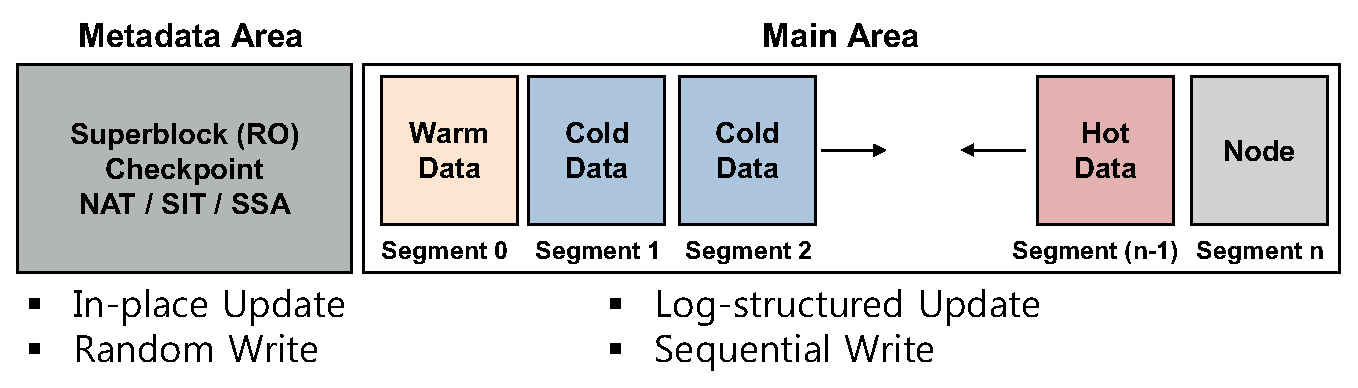
\includegraphics[width=3.2in]{./figure/f2fs_layout}
\caption{F2FS Partition Layout}
\label{fig:f2fs_layout}
\end{center}
\end{figure}

F2FS filesystem partition is composed of two areas. Metadata area keeps filesystem metadata and Main area keeps user generated data and node information where a node keeps file related metadata. Main area의 경우 2Mbyte 단위의 segment로 관리되며, 그림에 표현된 것과 같이, 데이터의 특성을 Warm data, Cold data, Hot data 그리고 Node로 구분하여 각기 다른 segment에 기록하도록 한다.

When the filesystem receives updates to existing data, it invalidates the data and appends the new data at the end of the segment. Log-structured filesystem은 이러한 정책을 통해 스토리지에 sequential 특성을 갖는 쓰기 요청을 전달할 수 있으며, 스토리지의 sequential 쓰기 성능을 활용할 수 있도록 한다. 그러나 업데이트가 발생했을 경우 기존의 데이터는 무효한 상태로 filesystem partition에 남게 되어 이들을 수거하는 정책이 필요하다. Thus, these systems spend considerable amount of time in reclaiming the space used by invalidated data blocks and copying valid blocks to pack the system. The process is called segment cleaning, and all log-structured systems suffer from the overhead of segment cleaning. F2FS filesystem의 경우 파일시스템 파티션에 free segment가 미리 정해놓은 특정 개수 이하로 감소했을 경우에 segment cleaning을 trigger한다. segment cleaning이 trigger되면, 파티션의 free segment와 현재 쓰기가 수행중인 segment를 제외한 나머지 segment 중에 victim segment 하나를 선정하여 cleaning을 수행한다. F2FS는 foreground segment cleaning과 Background segment cleaning의 2가지 cleaing 정책을 사용한다. Victim 선정 알고리즘은 foreground segment cleaning의 경우 greedy\cite{kawaguchi1995flash} 정책을, background segment cleaning의 경우 cost benefic\cite{rosenblum1992design} 정책을 사용한다. 
Victim segment를 선정하고 나면, victim segment 내의 유효 데이터들을 현재 쓰기가 진행중인 segment에 복사하고, victim segment를 free segment로 환원한다. 

Log-structured filesystem이 이와 같은 segment cleaning 동작을 수행하는 동안은 사용자의 입출력 명령을 수행할 수 없으므로, 파일시스템의 성능에 영향을 미치게 된다. Ever since Rosenblum et al introduced the concept of log-structured filesystem[12], all its descents such as JFFS\cite{woodhouse2001jffs}, YAFFS\cite{manning2010yaffs}, LogFS\cite{engel2005logfs}, F2FS\cite{lee2015f2fs} are inherent with the overhead.

\subsection{Garbage Collection and Flash Storage}

flash storage의 garbage collection에 대해 설명, multi-channel/multi-way의 경우 garbage collection에 대해서 설명

Flash memory 기반의 저장장치인 SSD에서도 log-structured filesystem의 segment cleaning과 유사한 garbage collection 동작이 필요하다. SSD가 전달받은 쓰기 명령을 out-of-place 방식으로 처리하는 FTL 계층으로 인하여, SSD 내에도 무효한 데이터들이 존재하게 된다. 이러한 데이터들로 인해 SSD의 empty space가 부족해지면 SSD level의 garbage collection 동작이 호출된다. SSD의 garbage collection 동작은 erase operation의 단위인 block 단위로 수행되며, 일반적으로 다음과 같은 step을 거친다. 먼저 free space로 환원할 victim block을 greedy victim selection 등과 같은 알고리즘을 이용해서 선택한다. greedy 방식의 경우, SSD 내의 블록들 중에서 가장 valid page 수가 적은 블록을 victim으로 선정하게 된다. Victim block이 선정되고 나면, block 내의 유효 데이터를 empty page로 복사한 뒤, 해당 block에 erase operation을 수행한다. 마지막으로 erase operation을 마친 block을 empty block으로 환원한다.

SSD가 여러개의 플래시 메모리와 multi-channel / multi-way로 구성될 경우 garbage collection 정책은 다양해 질 수 있다. Garbage collection 동작은 garbage collection을 수행 중인 Flash memory가 read/write operation을 처리하지 못하게 하므로, I/O 성능 하락의 주요 원인으로 작용한다. 그러나 SSD가 multi-channel로 구성되어 있을 경우, 특정 flash memory가 가비지 컬렉션을 수행중일 때, 해당 flash memory와 다른 채널에 연결된 flash memory 들을 통해 입출력 처리를 수행하도록 할 수 있다. 이러한 방식을 사용할 경우, SSD 내의 여유 공간 확보와 호스트로부터 전달받은 입출력 처리를 병렬적으로 함으로써, garbage collection 동작으로 인한 SSD의 성능 저하를 완화할 수 있다.

Superblock FTL\cite{kang2006superblock}은 SSD가 multi-channel / multi-way로 구성된 환경에서, 여러 개의 NAND block을 superblock으로 묶어 관리하는 기법을 제시한다. 각 channel, way에 연결된 flash memory에서 동일한 offset에 위치한 NAND block들을 하나의 superblock으로 관리한다. Superblock을 사용하는 SSD는 write operation을 전달 받으면, 먼저 empty superblock을 할당하여 데이터를 기록한다. 해당 superblock에 포함된 페이지들을 모두 기록하고 나면, 다음 empty superblock을 할당받아 write operation을 처리한다. 이와 같은 superblock 단위의 처리 방식은 SSD read/write operation이 자연스럽게 channel / way 병렬화를 활용할 수 있도록 한다. 더욱이 garbage collection 또한 superblock을 단위로 동작한다. superblock ftl에서의 garbage collection은 block 단위로 수행되는 garbage collection과 동작이 유사하며, 단지 victim block을 superblock 단위로 선정하고, 해당 superblock에 존재하는 유효 데이터들을 현재 쓰기가 수행중인 superblock으로 복사하도록 한다. Superblock 단위의 garbage collection은, SSD에 포함된 모든 flash memory가 garbage collection에 참여하도록 하므로, garbage collection 동작 수행 중에는 호스트의 입출력을 처리할 수 없는 단점을 갖는다.

\subsection{Log-structured Filesystem and SSD}

워크로드와 관계없이 모든 쓰기 요청을 sequential로 수행하는 Log-structured filesystem은 본디 Random write performance가 낮은 Hard Dist Drive의 성능을 끌어 내기 위해 고안되었다. 그러다 SSD와 같은 Flash memory based storage가 HDD 수요를 대체하기 시작하면서 다시금 Log-structured filesystem이 조명받기 시작하였는데, 이는 Log-structured filesystem의 쓰기 방식과 SSD의 쓰기 방식이 매우 흡사하기 때문이다. 위에서 언급했듯이, SSD는 Log-structured filesystem과 마찬가지로 FTL을 통해 out-of-place update를 수행하므로, Logical to Physical 매핑 정보를 유지해야 한다. FTL은 매핑 정보 관리 단위에 따라 Page-level FTL, Block FTL\cite{kim2002space}, Superblock FTL\cite{kang2006superblock}, 그리도 페이지와 블록 단위를 모두 사용하는 Hybrid FTL\cite{fast07}\cite{last08} 로 구분된다. 매핑 단위가 작을수록 Logical to Physical 할당이 유연하므로 Random write 워크로드에 대한 성능이 좋으나, 매핑 정보의 크기가 커지게 된다. 반대로 매핑 단위가 커질수록 더 작은 크기의 매핑 정보를 이용하여 파티션 관리가 가능하다는 장점이 있으나, Logical to Physical 할당이 자유롭지 못하여 Random write 워크로드에 취약한 특성을 갖는다. 이와 같은 성능상의 이유로 인해, Page 단위로 매핑을 관리하는 Page-level FTL이 일반적으로 사용된다. Page-level FTL은, 앞서 설명했듯이, Memory foot-print가 크다는 단점이 있으며, 따라서 메모리에 모든 매핑 정보를 올리지 않고, 매핑의 일부분 정보만을 메모리에 캐싱하여 사용하는 방식도 제안되었다\cite{dftl09}.

그러나 SSD가 받는 워크로드가 sequential로 한정되어 있다면, random write 성능을 위해 memory foot-print가 큰 page 단위 매핑을 사용할 필요가 없어진다. 대신 sequential 워크로드에서 좋은 성능을 낼 수 있는 block 단위 매핑을 사용함으로써, 성능 하락 없이 매핑 테이블 사이즈를 크게 줄일 수 있다. 만일 4KByte 페이지와 2MByte NAND 블록을 사용하는 256Gbyte SSD의 경우, Page-level FTL은 256MByte 크기의 매핑 테이블이 필요하나, Block FTL의 경우 단지 512KByte의 매핑 테이블이 필요하다. 이러한 점을 고려해 보았을 때, Log-structured filesystem을 사용함으로써 sequential 워크로드를 SSD에 전달할 수 있다면, SSD는 보다 작은 크기의 DRAM 만으로도 매핑 테이블을 관리할 수 있는 이득을 얻을 수 있게 된다.

\subsection{Layered Log-structured System}

When two log-structured systems stacked on top of each other, we call them as layered log system and an example of such system is illustrated in Fig \ref{fig:layered_log_system}. It shows that Flash based storage device is managed by log-structured file system. Virtual file system send data down to filesystem then the data is recorded in the filesystem partition. When there is not enough space left in the partition, the filesystem has to garbage collect the invalidate blocks. As a result, the filesystem has to send not only the data received from the virtual file system but also writes generated by the garbage collection.

Upon receiving the data from the filesystem, storage device records the updates on the storage medium. The location of the data is decided by the Flash Translation Layer (FTL), the software layer inside the SSD. Since erase operation in SSDs have large latency than program operation, all writes are not in-place updated but out of place updated just like the log structured filesystem and the existing data is invalidated. This out-of-place update behavior also calls for garbage collection. Thus, the final data written on the storage device includes both data received from the filesystem and writes generated from garbage collect of the device.

The storage device receives the data issued from Virtual File System along with more data as side effect of performing garbage collection on two layered log structured systems. As data is passed down to lower I/O layer, the size of data becomes larger and larger which is known as write amplification. Larger write amplification means trouble for SSDs because it not only has to handle more data but also reduces the life of the device.

Note that Logical to physical mapping information is mandatory in log structured systems. It is because every update is placed in elsewhere. The overhead of managing the mapping information is inverse proportional to unit size of the mapping and proportional to size of the log-structured partition. It is also important to note that both filesystem and storage device in layered log system has to maintain the mapping data, thus the memory overhead for the mapping information increases.


\begin{figure}[h]
\begin{center}
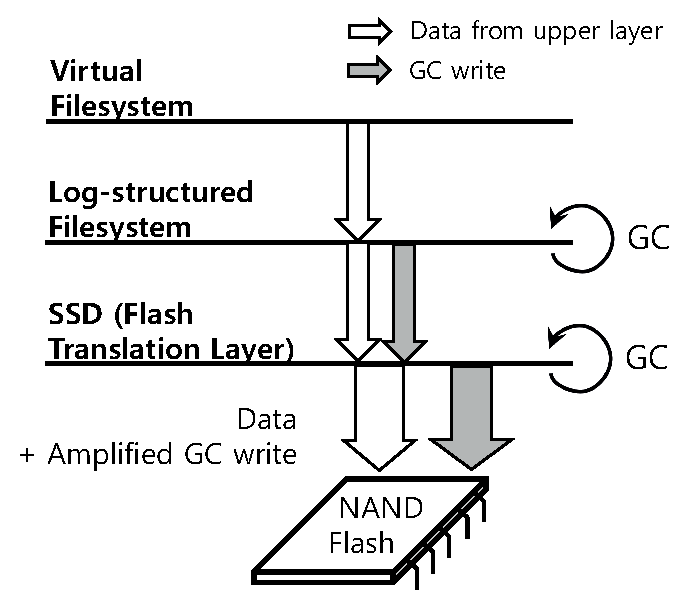
\includegraphics[width=2.5in]{./figure/layered_log_system}
\caption{Example of Layered Log System}
\label{fig:layered_log_system}
\end{center}
\end{figure}

\section{Garbage Collection Problem in Layered Log System}
\label{sec:CompoundGC}
\subsection{Definition}


Write Amplification cause a serious problem in layered log system, especially when garbage collection in storage device is triggered by the garbage collection of the file system. We name the behavior as compound garbage collection. We provide two case studies to describe its nature.

\subsection{Case Study 1: Uncoordinated Garbage Collection}
\label{subsec:case_study_2}

\begin{figure}[h]
\begin{center}
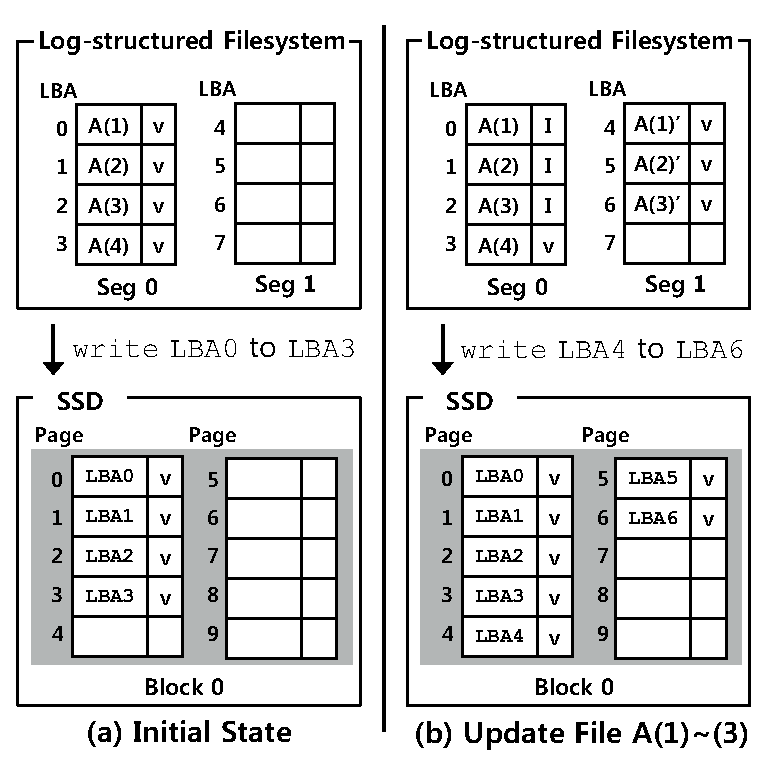
\includegraphics[width=2.9in]{./figure/comp_gc_scenario_2}
\caption{Example of Uncoordinated Garbage Collection}
\label{fig:comp_gc_2}
\end{center}
\end{figure}

로그 기반의 시스템은 기존에 저장된 데이터에 업데이트가 발생했을 때, 업데이트된 데이터를 파티션의 빈 영역에 기록하고 기존 데이터를 무효 처리(Invalidation)한다. 이러한 로그 시스템이 중첩될 경우에는, 데이터의 유효 상태가 상위 로그 계층과 하위 로그 계층에 서로 다르게 나타날 수 있다. Fig \ref{fig:comp_gc_2} 는 이러한 경우를 보여준다. Log-structured filesystem 에서 세그먼트 0에는 LBA 0$\sim$3, 세그먼트 1에는 LBA 4$\sim$7에 해당하는 데이터를 저장한다고 가정하자. SSD는 하나의 블록에 10개의 페이지를 가지며, 예제의 단순화를 위하여 하나의 페이지에 하나의 LBA에 해당하는 데이터를 기록한다고 가정하자. Fig \ref{fig:comp_gc_2}-(a)는 File `A'가 시스템에 저장된 상황을 파일시스템과 SSD 각각에 대해 보여준다. File A는 4개 Logical Block 크기이며, 파일시스템에서 A(1)$\sim$A(4)로 나뉘어 LBA0$\sim$LBA3에 할당되어 있다. 따라서 파일시스템은 LBA0부터 LBA3까지 4개 Logical Block에 대한 쓰기 명령을 SSD에 전달하며, SSD는 4개 LBA를 Block 0의 Page 0$\sim$3에 할당하여 저장하였다. 이어서 Fig \ref{fig:comp_gc_2}-(b)는 File A(1)$\sim$A(3)가 업데이트된 상황을 보여준다. Log-structured Filesystem 이므로 업데이트가 발생한 File A(1)'$\sim$A(3)'을 비어있는 LBA4$\sim$6에 기록하고, LBA0$\sim$2에 저장된 기존의 데이터는 Invalidation 한다. 파일시스템은 새로 데이터를 기록한 LBA4$\sim$6에 대한 쓰기 명령을 SSD로 전달하며, SSD는 이를 Page 4$\sim$6에 기록한다. 주목해야할 점은, SSD의 입장에서는 파일시스템으로부터 전달받은 LBA4$\sim$6에 대한 쓰기 명령이 기존에 SSD에 저장된 LBA0$\sim$2에 대한 overwrite이라는 정보를 알 수 없다는 점이다. 따라서 SSD의 Page 0$\sim$2에 기록된 LBA0$\sim$2 데이터는 유효한 상태로 남게 된다.

만일 이와 같은 상황에서 각 계층에서 garbage collection이 호출된다면, 파일시스템 계층에서는 업데이트로 인해 Invalidation된 File A(1)$\sim$(3)에 할당된 LBA 영역을 수거할 수 있을 것이다. 그러나 SSD 계층에서는 LBA0$\sim$2이 저장된 페이지가 유효하게 남아있으므로, 공간을 수거할 수 없으며, 오히려 경우에 따라 해당 페이지에 대한 복사 동작이 일어날 수 있다. 이와 같이, 파일시스템과 SSD의 상태정보가 서로 다름으로써, 디바이스단의 가비지 컬렉션 동작에서 이미 파일시스템에서는 무효화된 페이지에 대한 복사 동작이 발생하는 경우를 우리는 uncoordinated garbage collection이라 하였다.

Uncoordinated garbage collection 문제는 TRIM Command\cite{shu2007data}를 통해 완화될 수 있다. TRIM Command는 파일시스템이 무효화된 LBA 영역을 SSD에 전달해주는 SATA Command이다. TRIM Command를 전달받은 SSD는 파일시스템이 TRIM Command를 통해 전달한 LBA 영역을 SSD 메타데이터에서 Invalidation 함으로써, SSD 레벨의 가비지 컬렉션 동작에서 불필요한 페이지 복사 동작을 줄일 수 있다. 그러나 TRIM Command를 사용하는 경우에도 uncoordinated garbage collection은 여전히 발생할 수 있다. 그 이유는 파일시스템이 TRIM Command를 Invalid LBA가 발생할 때마다 보내지 않기 때문이다. 일례로, Log-structured 파일시스템인 F2FS의 경우, 파일시스템 복구 시 사용하는 checkpoint를 파일시스템 파티션에 기록할 때에 TRIM Command를 SSD로 보낸다. 다시 말해, F2FS가 checkpoint를 수행하기 전까지는, SSD는 파일시스템에서 무효화된 LBA 영역 정보를 받을 수 없다. 즉, TRIM Command는 SSD의 불필요한 유효 페이지 복사 Overhead를 감소시킬 수 있으나, 파일시스템의 TRIM Command 사용 정책에 따라 여전히 Uncoordinated garbage collection 문제가 발생할 수 있다. 추후 Uncoordinated Garbage Collection으로 인한 성능저하 결과는 Section \ref{subsec:io_performance}에서 보여준다.


\begin{figure*}[t]
\begin{center}
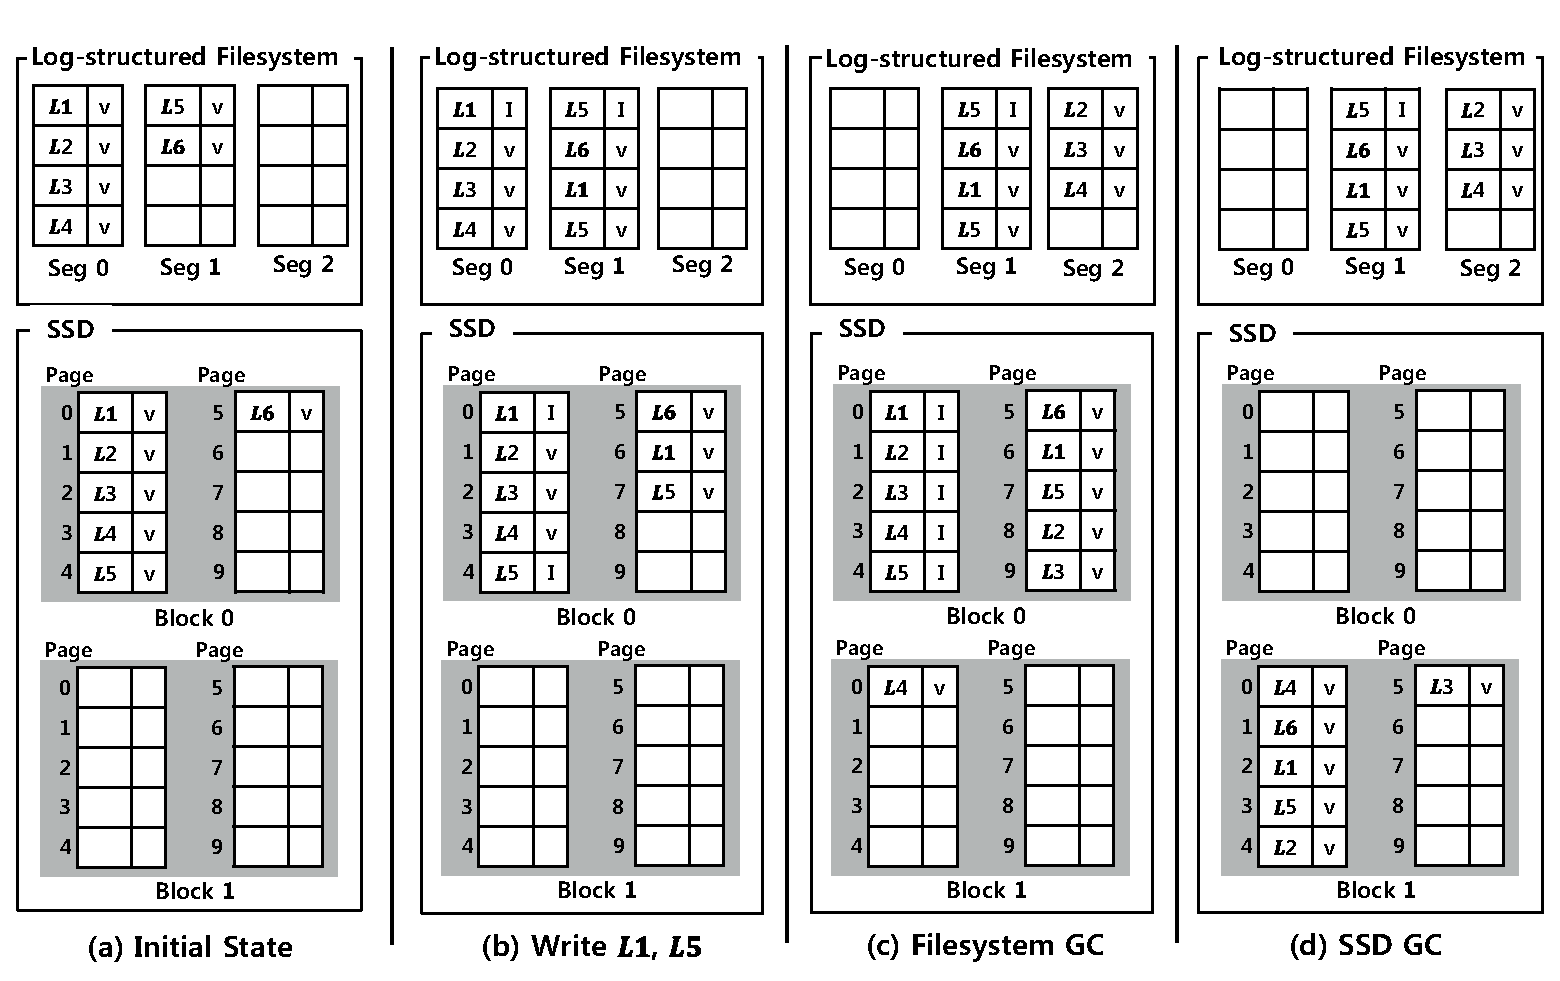
\includegraphics[width=6in]{./figure/comp_gc_scenario_1}
\caption{Example of Compound Garbage Collection}
\label{fig:comp_gc_1}
\end{center}
\end{figure*}

\subsection{Case Study 2: Compound Garbage Collection}
\label{subsec:case_study_1}

We define compound garbage collection as the case where the lower level log system performs garbage collection on data blocks which are already garbage collected by the higher level log system. Fig \ref{fig:comp_gc_1} illustrates a scenario of compound garbage collection.

Before we begin to describe how compound garbage collection works, we make following assumptions. Each segment on a filesystem has four pages and the filesystem performs garbage collection in units of segments. We assume that segments that are not depicted in Fig \ref{fig:comp_gc_1} are filled with cold data. Each block on a SSD contains 10 pages and the SSD performs garbage collection when only one empty segments and only one empty block is available on the layer, respectively. 추가적으로, 파일시스템에서 무효화된 LBA 영역은 TRIM Command를 통해 SSD가 알 수 있다고 가정한다.

Each page in the filesystem and the SSD in Fig \ref{fig:comp_gc_1} keeps the LBA (Logical Block Address) of its respective page and a flag to note validity of the page. 그림에서 LBA는 간략히 `$L$'로 표기하였다. 예를 들어 `$L1$'는 LBA1를 의미한다. The flag has two values: V indicates that the page is valid and I indicates invalid. Let’s further assume that segment 0 holds data pages for LBA 1 to 4 ($L1$$\sim$$L4$)and segment 1 contains LBA 5 and 6($L5$ and $L6$).  Both segments are stored in block 0 on our SSD. Note that all the flags on the filesystem and the SSD shows that all the data is valid.

Fig \ref{fig:comp_gc_1}-2 shows the state of the filesystem and the SSD after LBA 1 and 5 is updated. Since both layers are log-structured systems, updated data is appended to the end of each system. The flags in old pages of the filesystem and SSD are set to invalid. Upon receiving a update and writing a new data on segment2, the filesystem detects that there is only one segment in the system, and thus decides to garbage collect. Fig \ref{fig:comp_gc_1}-3 shows the status of each layer after the filesystem garbage collection. For example we assume that the filesystem selects segment 0 as the victim segment. Valid pages in segment 0 that is LBA 2 to 4 are copied to available empty segment 2. The filesystem notifies the changes in the system to the storage device, and then the SSD has to reflect the changes made to LBA 2 to 4 by invalidating pages mapped for LBA 2 to 4 and make a new copy of the data to block 0. When the device begins to write LBA 4 to the last page of block 0, it detects that there is only one empty block in the storage system, thus the storage level garbage collection takes a place. Fig \ref{fig:comp_gc_1}-4 shows the system status after the garbage collection. Recall that, all the other blocks in the storage are filled with cold data, thus block 0 is selected as the victim for the garbage collection.  All the valid pages in block 0 is copied to empty block 1.

There are two things to note in our first case study. First, storage level garbage collection is triggered as a result of filesystem level garbage collection. Second, filesystem and storage system relocates pages with LBA 2 to 4 in the course of garbage collecting segment 0 and block 0, respectively. Recursive garbage collection on the filesystem and the storage system forces to rewrite the same data over and over. Such compound garbage collection acts as a factor that increases Write Amplification Factor (WAF) in SSDs.


\subsection{Case Study 3: Multi-streams Sequential Write (실험 필요)}


\section{Unified Storage Layer}
\label{sec:USL}

In this paper we propose Unified Storage Layer to address compounded garbage collection in log systems. Unified Storage Layer keeps two LBA regions on filesystem layer depending on I/O characteristics of the filesystem. On one of the regions filesystem has control over when to perform garbage collection for both filesystem and SSD, thus SSD does not have to garbage collect on its own.


\subsection{Design}

Fig \ref{fig:f2fs_layout}에서 언급했듯이, F2FS는 filesystem의 메타데이터를 관리하기 위한 영역(Metadata area)과 User data와 File releated metadata를 관리하는 영역(Main area)로 나누어 진다. Note that each area exhibits different write patterns. Since metadata area handles all writes in in-place update manner, the region show random write pattern. On the contrary, data and node in main area is written in log-structured style which shows sequential write pattern.

Note that F2FS is flash friendly filesystem and tries to reduce storage I/O overhead by sending large units of data. For example, unit of garbage collection for main area is section which is 2MByte in size. In fact, the main area does not perform in-place update unless it is necessary and unit of garbage collection is large resembles characteristics of SSDs. The size of metadata and main areas are determined by the size of the partition, the size cannot be altered after formatting a partition.

After reviewing the filesystem features and the I/O characteristics of each area, we came up with an idea to solve the uncoordinated garbage collections on log system. The crux of Unified Storage Layer is to manage LBAs with disaggregate mapping, which is a mapping specifically tailored for Unified Storage Layer. Disaggregate mapping which is shown in Fig \ref{fig:da_mapping_layout} keeps two different mapping schemes. Metadata area is managed in page mapping and LBs in main area are one-to-one mapped with PBAs in SSD.


\begin{figure}[h]
\begin{center}
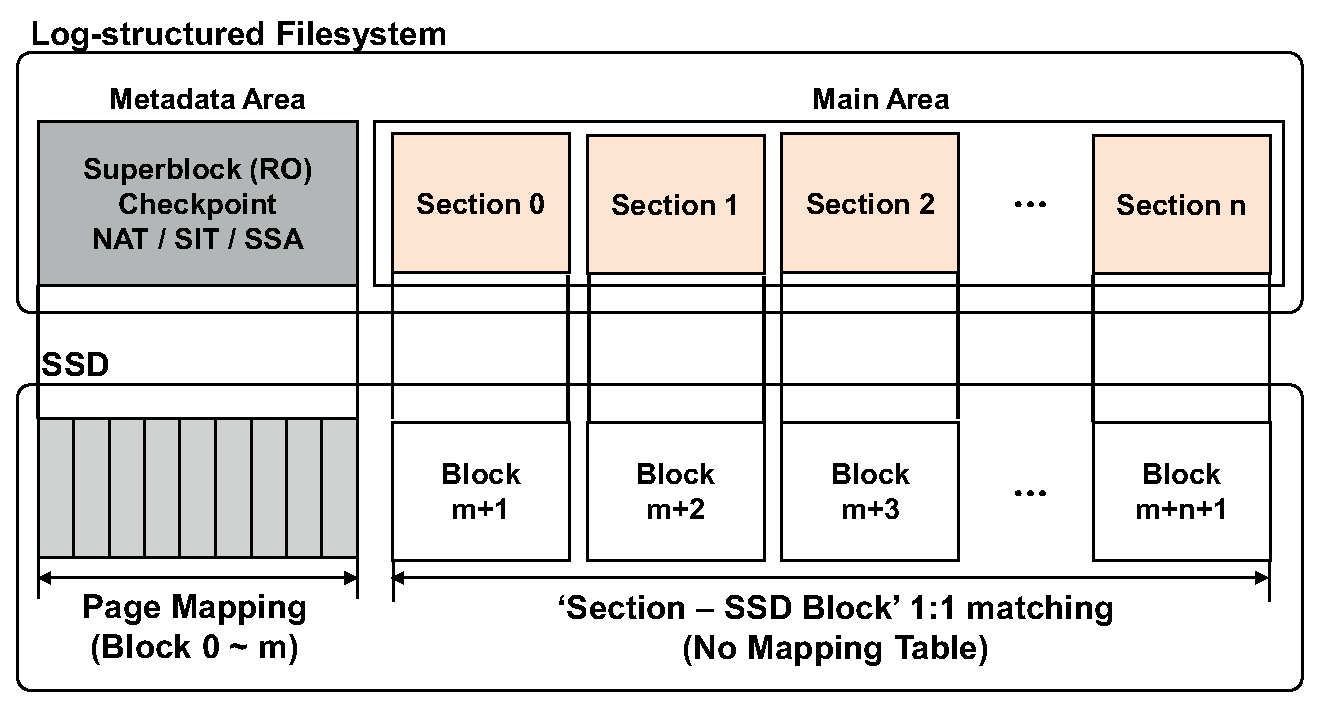
\includegraphics[width=3.2in]{./figure/usl_layout}
\caption{Disaggregate Mapping Layout}
\label{fig:da_mapping_layout}
\end{center}
\end{figure}


Since the SSD knows the area information of F2FS in Unified Storage Layer, the SSD distinguishes LBA requested by the filesystem is for the main area or for the metadata area. The filesystem metadata is stored in page mapped region of the SSD and LBAs for filesystem main area, $LBA_i$, is directly mapped with corresponding PBAs in the SSD, $PBA_j$, where i=\{1…n\} and j=\{1…n\}.

Each section in main area is matched with a block in the SSD. Thus, the update in a section is applied to the corresponding block in the SSD. By mapping sections to physical blocks, that is `$section_l\big|_{l=1...x}=block_{m+1}\big|_{m=1...x}$', the memory overhead of managing mapping table can be removed. There are two layer, that is filesystem and Unified Flash storage layer, and the following sections describes each layer in more detail.

\subsection{Filesystem Layer}
\label{subsec:fs_layer}

The filesystem in Unified Storage Layer plays two important roles. First is to persistently record the user data received from the virtual filesystem layer after recording the data to the filesystem partition. Second is to handle garbage collection on main area and send set of empty section numbers acquired from garbage collection process to the storage. Upon receiving the section numbers the SSD makes the corresponding blocks as empty blocks. Therefore, there is no need to garbage collect the blocks in main area but to erase the target blocks that the filesystem requested. 
In order to fulfill the task of the filesystem in Unified Storage Layer, we modified F2FS, the log-structured filesystem. 

First, we modified garbage collection policy of the filesystem and second, we introduce patch manager to avoid partial writes and finally, we added a mechanism to transfer section numbers reclaimed by garbage collection to the storage device. Although F2FS is known as log-structured, strictly speaking it is more like hybrid version of log-structured and in-place update filesystem. When there is enough space in the partition, F2FS appends all writes, however, when the available space goes under certain threshold, F2FS uses Slack Space Recycling (SSR), which in-place updates a new data on invalided pages on SSD. F2FS exploits SSR to delay the garbage collection from happening and also reduces WAF in filesystem layer. However SSR in F2FS means in-place update with random write on sections in main area. 파일 시스템의 section과 SSD의 block이 1:1로 매핑되어 있는 Unified Storage Layer에서는, SSR로 인하여 section에 random write이 발생하게 되면 그 section에 할당된 NAND block에 random write을 유발한다. As a result some of the writes on a SSD block cannot be written because of NAND program protocol. In order to guarantee that writes to main area are sequential writes, we disabled the use of SSR in the filesystem.

\begin{figure}[h]
\begin{center}
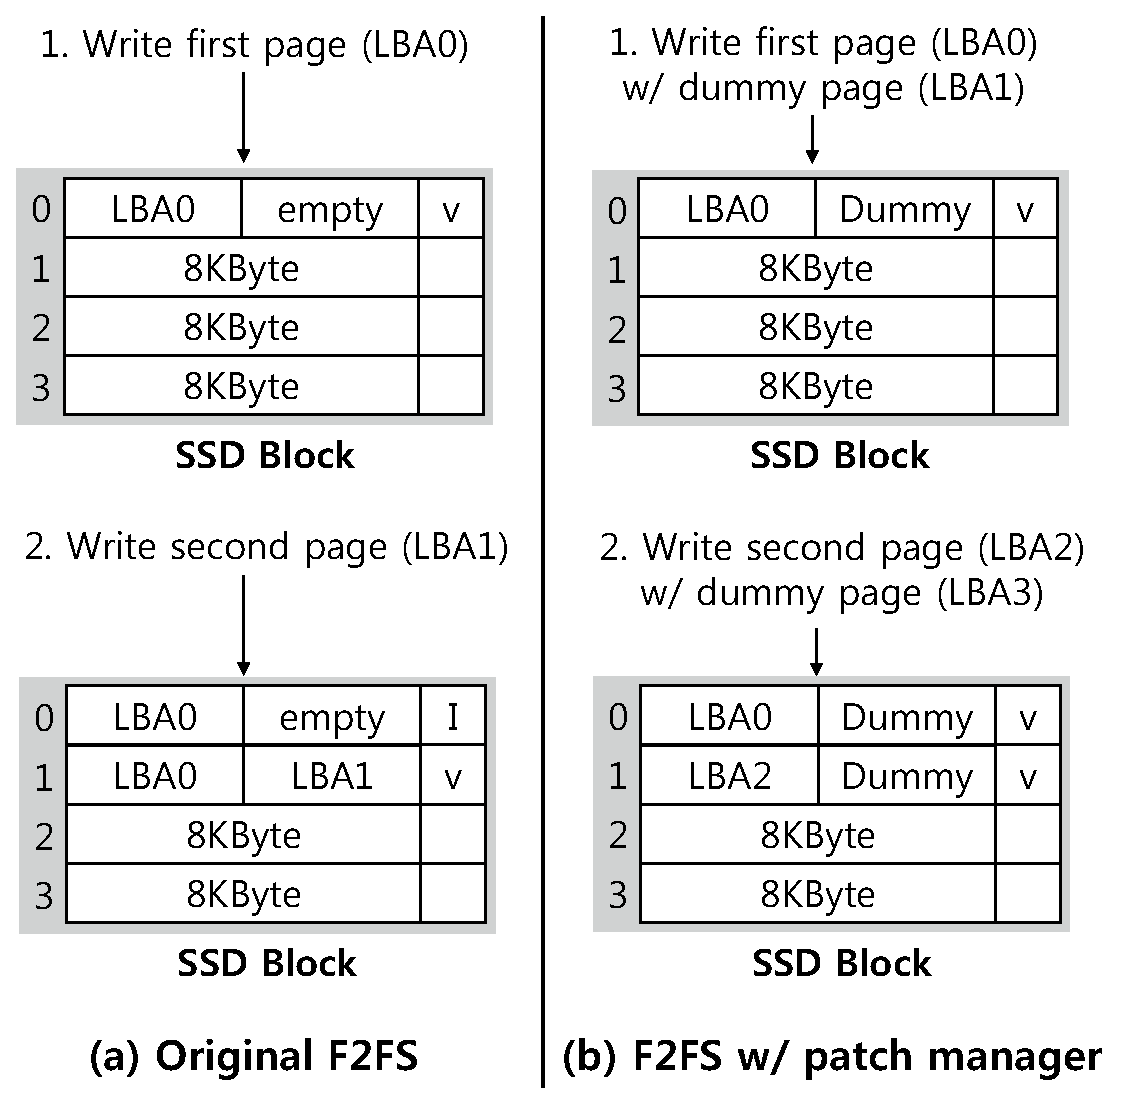
\includegraphics[width=3in]{./figure/patch_manager_ex}
\caption{Two-page write behavior w/ and w/o patch manager}
\label{fig:patch_manager_ex}
\end{center}
\end{figure}

When a SSD receives a write request that is smaller than the page size of the SSD, the device writes the data using partial write on a page which wastes the rest of the page. F2FS has unit size of 4Kbyte and requests multiples of the unit size to the storage device. On the other hand, the page size of SSDs varies from 4Kbyte, 8Kbyte, and to 16Kbyte, depending on the manufactories. If the unit size of write in filesystem and SSD is not aligned to each other, there is no other way but to use partial write on SSD. Fig \ref{fig:patch_manager_ex}-(a) illustrates the second issue in F2FS where SSD uses 8Kbyte as page size.

F2FS allocates a LBA on every 4Kbyte, and a SSD block in Fig \ref{fig:patch_manager_ex} is composed of four 8Kbyte pages, and each page is numbered and also has a flag to indicate validity of corresponding page. Upon receive a write request for LBA0 from the filesystem, the SSD programs it on page 0. Since the page is larger than the size of request, the SSD partially programs the page with the request and the rest of 4Kbyte in the page is left empty.

Let’s assume that after sometime, the filesystem sends another request to LBA1. Since LBA1 is logically consecutive to LBA0, the two LBAs can fit in a page of the SSD. Although page0 has empty space, LBA1 cannot be placed in there because of NAND programming protocol. In ordinary SSDs, the LBA0 in page0 is internally copied to the buffer and then copied to page 1 with LAB1.

In Unified Storage Layer, LBA1 cannot be placed on page 1 because Unified Storage Layer does not keep a mapping table for main area, instead each PBA have matching LBA. First and second 4Kbyte of page1 is designated for LBA2 and LBA3, respectively. In order to address the side effect of removing mapping information from the SSD, we introduce Patch Manager in the filesystem which mandates each write request to be aligned to the page size of the SSD. Fig \ref{fig:patch_manager} shows location of Patch Manager in the I/O hierarchy. The main role is to align the size of all requests from the filesystem to the page size of the SSD. The filesystem exploits bio structure to form a request to the storage, but before sending it to the storage, the filesystem sends it to Patch Manager to check whether the request is aligned with the page. If it is aligned, then it simply returns bio structure. And if it is not aligned, then Patch Manager adds a dummy page and makes the length of the request aligned with the page size. Since a dummy page does not contain any useful data, we mark the page with dummy data as invalid to let garbage collection reclaim the page.


\begin{figure}[h]
\begin{center}
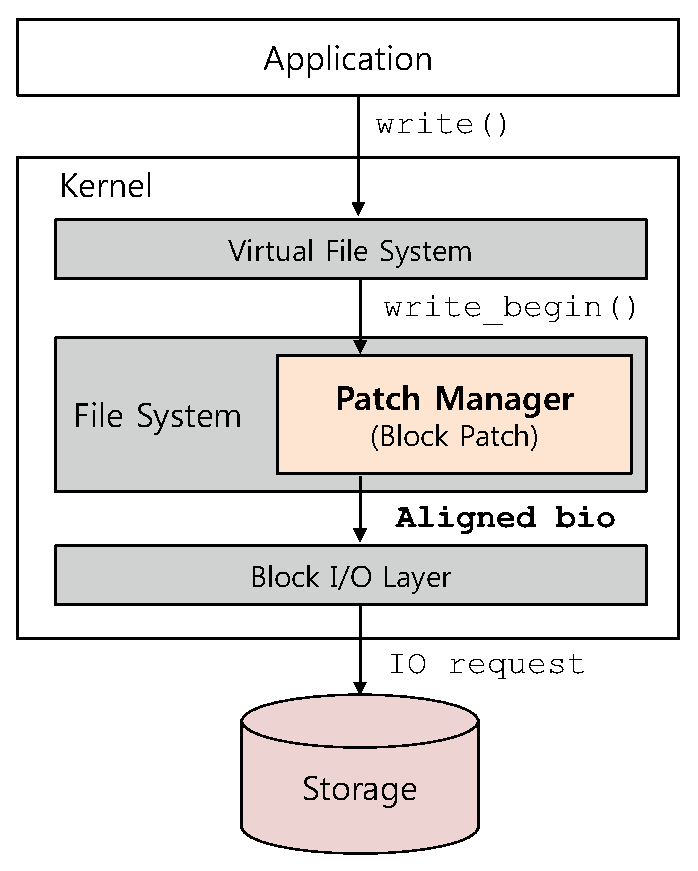
\includegraphics[width=2in]{./figure/patch_manager}
\caption{Block Patch Manager}
\label{fig:patch_manager}
\end{center}
\end{figure}

Fig \ref{fig:patch_manager_ex}-(b) shows how patch manager works in Unified Storage Layer. Upon receiving a write request to LBA0, patch manager detects that the request is not aligned to 8Kbyte, thus patch manger adds dummy 4Kbyte page along with LBA0 to the SSD. The storage device assigns LBA1 to the dummy data and programs all the data on page 0. The filesystem assigns the next logically consecutive request to LBA2. Since the request for LBA2 is also not aligned, Patch Manager also adds dummy page to the request and writes the request in page 1.

With the help of Patch Manager, Unified Storage Layer achieves the goal of mapping each LBA to PBA in storage systems. However, one may point out a problem of increased WAF in filesystem layer because of the additional of dummy page. Our experiment shows that Patch Manager added only handful of dummy pages. It is because most of writes in filesystem were in multiples of page size.

Finally, Unified Storage Layer requires a means to transfer the acquired set of section numbers from filesystem garbage collection process to the storage device. Since all PBAs are matched to LBAs of main area of F2FS, SSD does not perform garbage collection on those blocks; instead the filesystem performs garbage collection and sends the number of sections to erase in the SSD. The technique to send section numbers described in the following section.


\subsection{Unified Flash Storage}
\label{subsec:flash_storage}

Unlike SSDs with page mapping or other hybrid mapping schemes, the storage device used in Unified Storage Layer does not keep mapping information for main area of the filesystem. Unified Flash Storage is defined as storage in Unified Storage Layer which uses disaggregated mapping scheme. It is combination of page mapping for metadata area and no mapping scheme for main area of the filesystem. By making the size of section in filesystem same as the size of block in SSD and each section be one-to-one linked to a physical block, it is able to eliminate the use of mapping schemes. There are at least two significant benefit of using disaggregate mapping. First is that it removes the overhead of garbage collection in main area, and second is that it has very low memory footprint. For example, page mapping, which is most widely used mapping scheme, creates 1Gbyte of mapping information in memory.

As we mentioned in section \ref{subsec:fs_layer}, filesystem $section_l\big|_{l=1...x} is fixed to SSD =block_{m+1}\big|_{m=1...x}$, and filesystem and SSD uses same unit from write data called a page. Note that filesystem uses 4Kbyte page and SSD uses 8Kbyte page in Unified Storage Layer. To prevent the orders of LBAs within the block from chaning, especially when the size of physical page is larger than the size of LBA, we use Patch Manager to fill in dummy data. By matching sections to blocks and using Patch Manager, we are able to make garbage collection free NAND Flash based storage device, at least for the main are of the filesystem. The storage device needs to just erase blocks upon receiving section numbers from the filesystem. The interface we used in transferring section numbers is write system call. To distinguish ordinary write calls from sending section numbers, we used numbers beyond the maximum available LBA in filesystem partition. Thus when SSD receives LBA number larger than the size of flesystem partition, the firmware of SSD recognizes the write call as means to inform section numbers to erase. The storage system simply erases blocks upon receiving the section numbers. 


\begin{figure}[h]
\begin{center}
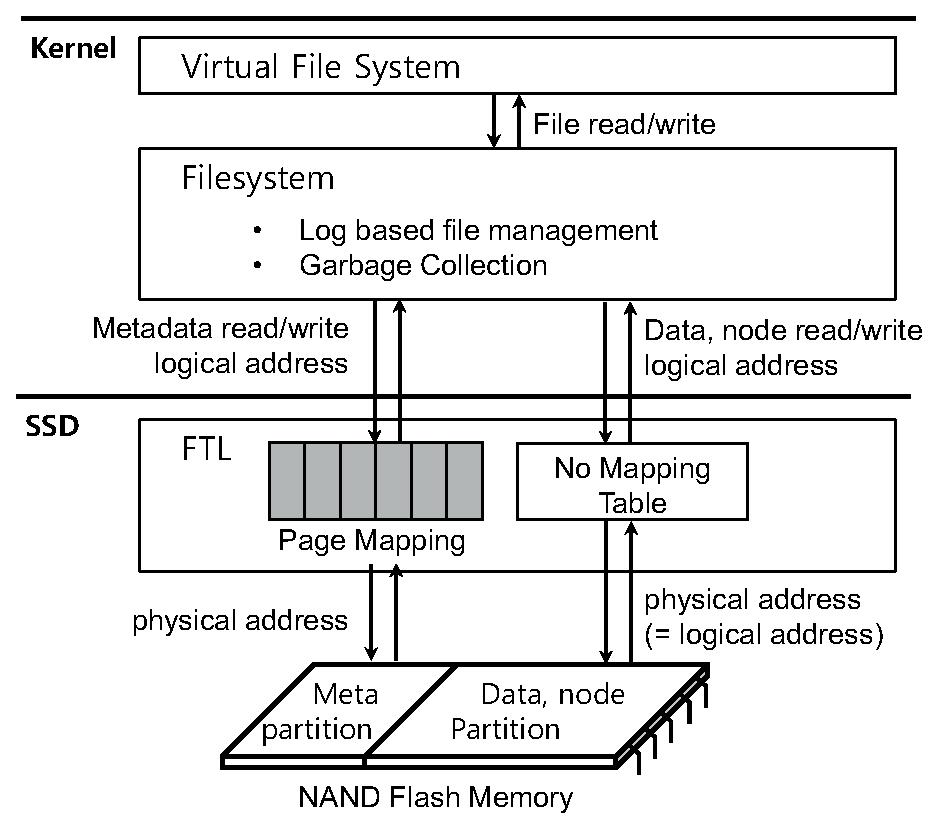
\includegraphics[width=3in]{./figure/usl_architecture}
\caption{System with Unified Storage Layer}
\label{fig:usl_layout}
\end{center}
\end{figure}

Fig. \ref{fig:usl_layout} illustrates the system layer with Unified Storage Layer. Firmware makes decision over received LBAs. If they are for metadata area, the firmware directs them to page mapping managed region of SSD; If LBAs within the range of main area is received, the firmware recognizes the LBA as PBA, and programs to respective block; When the firmware receives LBA Larger than system partition, it computes to find block number to erase instead of garbage collecting the storage device.


\section{Write Amplification Analytic Model}
\label{sec:WA_model}


%5장의 존재 의미
Write amplification은 user page write 횟수에 대한 실제 page write의 평균 횟수이다.
이는 NAND flash의 inplace update가 불가능한 특성때문에 발생하며, SSD의 성능을 결정짓는 원인 중에 하나이다. 
Write amplification을 모델링함으로써 SSD의 현재 성능을 이해하고, 이를 바탕으로 성능 발전의 방향을 잡을 수 있다.
또한, SSD가 정상적으로 작동하고 있는지를 판단할 수 있는 지표로 활용할 수도 있다.


%기존의 WAF analytic model
SSD의 write amplificaion을 수학적으로 모델링 하기 위한 연구가 많이 진행되고 있다. 
Xiao-Yu Hu\cite{Hu:2009:WAA:1534530.1534544}\cite{Hu:2010:RZ3771}는 SSD에서 발생하는 random write를 the coupon collector's problem에 근사시켜서 write amplification을 모델링하였다. 
Ragiv Agarwal\cite{Agarwal5700261}은 write가 uniform distributed random으로 발생할 경우, 모든 block에 같은 수의 invalid page가 저장되어 있다고 가정하고 모델링하였다.
Xiang Luojie\cite{Luojie6167472}는 Ragiv Agarwal의 모델을 발전시켰다.
하나의 page가 무효화 될 확률을 구하고, 이를 이용하여 한 블록의 invalid page수를 구하여 모델링하였다.
Peter Desnoyers\cite{Desnoyers:2012:AMS:2367589.2367603}는 Markov chain을, Benny Van Houdt\cite{VanHoudt2013}는 mean field model을 이용하여 모델링을 하였다.


%사용한 모델, 가정한 내용
우리는 write amplification의 이론값 계산을 위해 Desnoyers\cite{Desnoyers:2012:AMS:2367589.2367603}의 모델을 사용하였다.
그 중에서도 우리와 유사한 환경인 uniform traffic과 greedy cleaning을 사용하는 모델을 사용하였다.
이 모델은 SSD의 wear-leveling과 채널/웨이에 의해 발생할 수 있는 부차적인 효과를 무시하였다.
Traffic은 uniformly distributed이고, 모든 write는 page크기 단위이다.
이 모델에서의 Write amplification A는 다음과 같다.


%수식 작성 및 인자설명
\begin{equation}
\label{analy_grd_unif_wa}
A=\frac{n_p}{n_p-(X_0-1)}
\end{equation}
여기서 $n_p$는 number of pages per block 이고, $X_0$는 다음과 같다.

%alpha
%\begin{equation}
%\label{analy_grd_unif_X0}
%X_0=\frac{1}{2}-\frac{n_p}{\alpha}\mbox{W}\left( -(1+\frac{1}{2n_p})\alpha e^{-(1+\frac{1}{2n_p})\alpha}\right)
%\end{equation}

%rho
\begin{equation}
\label{analy_grd_unif_X0_rho}
X_0=\frac{1}{2}-\frac{n_p}{\rho+1}\mbox{W}\left( -(1+\frac{1}{2n_p})(\rho+1)e^{-(1+\frac{1}{2n_p})(\rho+1)}\right)
\end{equation}

여기서 $\mbox{W}()$는 Lambert W function\cite{Corless:BF02124750}이다. 
$\rho$는 overprovisioning factor로 $T$(\# of physical blocks)와 $U$(\# of user blocks)에 대하여 $\rho=\frac{T-U}{U}$의 값을 가진다.


\section{Experiment}

\subsection{Experiment Setup}
\label{subsec:exp_setup}


Table \ref{tab:ssd_info} shows specification of SSD used in the performance evaluations. The total available capacity is 256Gbyte with 23.4Gbyte overprovisioning, and with 8Kbyte page. The SSD performs garbage collection in units of superblock with size of 256MByte where superblock is group of Flash blocks with same way number in array of flashes channel.

\begin{table}[h]
\begin{center}
\begin{tabular}{|c|r|r|} \hline
Parameter			& Specification 				\\ \hline\hline
Capacity			& 256 Gbyte 				 	\\ \hline
Overprovisioning	& 23.4 Gbyte					\\ \hline
Page size			& 8 Kbyte						\\ \hline
Block size		& 4 Mbyte						\\ \hline
Superblock size	& 256 Mbyte					\\ \hline
\# of Channel		& 4 							\\ \hline
\# of Way			& 4 							\\ \hline
\# of Plain		& 4 							\\ \hline


\end{tabular}
\end{center}
\caption{SSD Specification}
\label{tab:ssd_info}
\end{table}

Table \ref{tab:system_info} shows mapping mechanism used for filesystem and SSD. Layered Log System(LLS) uses F2FS in kernel 3.18.1 as the base filesystem and page mapping in SSD. In-place Update System (INP)의 경우 대표적인 In-place update 방식의 Ext4 파일시스템을 page 단위 mapping table을 관리하는 SSD 위에서 동작시키도록 하였다.. Unified Storage Layer(USL) uses F2FS DA and disaggregate mapping for filesystem and SSD, respectively.

\begin{table}[h]
\begin{center}
\begin{tabular}{|c|c|c|c|} \hline
				& LLS	& INP	& USL 				\\ \hline\hline
Filesystem		& F2FS	& Ext4	& Unified FS			\\ \hline
SSD Mapping		& Page	& Page	& Disaggregate		\\ \hline
\end{tabular}
\end{center}
\caption{System Information (Filesystem and SSD Mapping scheme)}
\label{tab:system_info}
\end{table}


\subsection{The size of mapping information}

Table \ref{tab:meta_size} compares the size of mapping tables in different mapping schemes. Assume that all schemes use the SSD descried in Table 1. 

\begin{table}[h]
\begin{center}
\begin{tabular}{|c|r|} \hline
									& Mapping Size	\\ \hline\hline
Page mapping							& 256 Mbyte		\\ \hline
FSDV\cite{zhangremoving}				& $\leq$	256 Mbyte		\\ \hline
Hybrid mapping (LAST \cite{last08})		& 4 Mbyte			\\ \hline
Disaggregate Mapping 					& 1 Mbyte			\\ \hline
\end{tabular}
\end{center}
\caption{The size of Mapping table (256GByte SSD)}
\label{tab:meta_size}
\end{table}

Page mapping uses 256Mbyte of memory where disaggregate mapping uses only 1Mbyte. Although page mapping has large memory footprint, its most valuable characteristics is that data can be places in any available places in the storage. However, as the size of SSDs is increasing, merits in using page mapping is becoming less appealing. For example, 1TByte and 4TByte SSD with 4Kbyte page size capacity need 1Gbyte and 4Gbyte of memory to hold the mapping information.

FSDV(File System De-Virtualizer\cite{zhangremoving})은 Filesystem의 매핑 정보가 SSD의 physical address를 가리키도록 하고, 그에 해당하는 SSD의 매핑 entry를 제거함으로써 SSD의 매핑 테이블 크기를 dynamic하게 조절하는 기법이다. 그러나 worst case의 경우 기존 페이지 매핑 방식과 동일한 크기인 256 Mbyte의 매핑 테이블을 SSD가 관리해야 한다. VFSL(Virtualized Flash Storage Layer\cite{josephson2010dfs})는 Logical to Physcial 매핑 정보를 SSD의 FTL이 아닌, 호스트의 Device Driver 단에서 관리하는 기법이다. VFSL은 호스트에서 매핑 정보를 관리하므로, 호스트의 CPU, 메모리 자원을 활용할 수 있는 장점을 갖으나, 매핑 테이블 크기는 이득이 발생하지 않으므로, 여전히 큰 매핑 정보 관리 overhead가 발생한다. FSDV와 VFSL에 대한 자세한 설명은 \ref{related_works}에 기술되어 있다.

Disaggregate mapping uses page mapping for the region allocated for metadata area of filesystem and keeps no mapping information for the main area. the memory foot print is only 1Mbyte which consumes about 256 times less than that of page mapping. Segment bitmap, Buffered Segment Number 등 USL의 스토리지가 동작하기 위한 추가적인 메타데이터를 모두 합할 경우에도 그 크기는 약 4.73MByte 이다. 이는 하이브리드 매핑 FTL인 LAST의 매핑 테이블 크기와 비슷한 수준이며, 페이지 단위 매핑 테이블의 약 54분의 1의 크기이다. 더욱이 Disaggregate mapping의 메타데이터 크기는 파티션 크기가 고정되면 변경되지 않으므로, 작은 크기의 메모리를 SSD에 탑재하는 것이 가능하다.



\subsection{Removing the Garbage collection overhead}

In section \ref{sec:CompoundGC} we describe a case where compound garbage collection becomes a problem. We use the case scenario to measure the performance of Unified Storage Layer.

Since SSDs are sensitive to test environment, we create a precondition prior to performing any experiments. First, we format and create a partition using available 256Gbyte of space. Next, we create 170Gbyte file using sequential buffered write operation and flushed the dirty pages in page cache using fsync() system call. Then we perform 4Kbyte buffered random write on created file. Single iteration of random write overwrites 85Gbyte of the file starting from 0 to 85GByte LBAs of the file. We measure the performance and WAF on each iteration and Fig \ref{fig:170_85_randw} shows the result. 



\begin{figure*}[t]
\label{fig:170_85_randw}
\centering

\subfigure[Filesystem WAF]{
 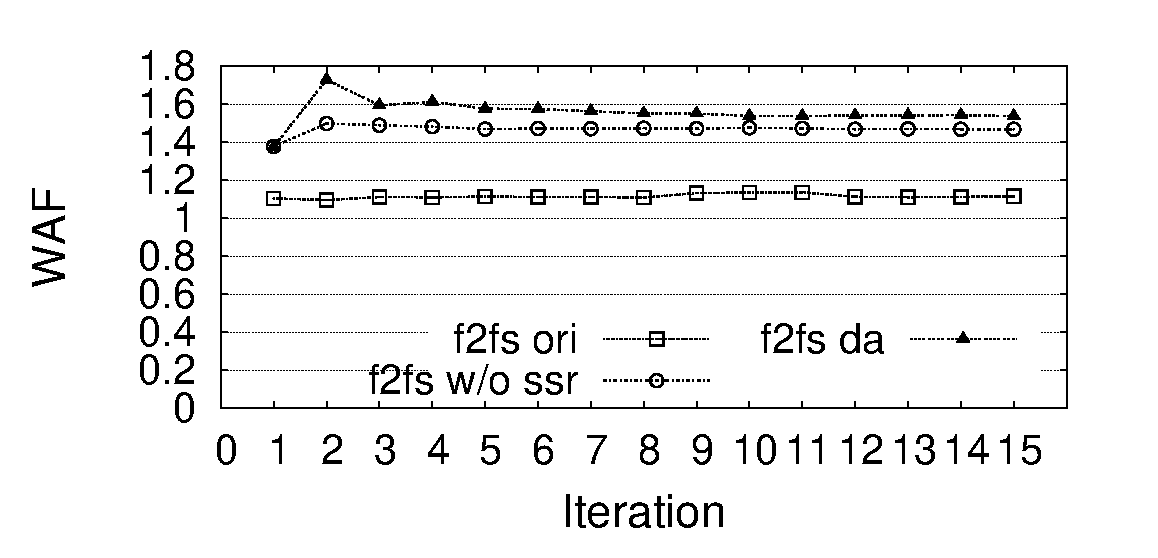
\includegraphics[width=3in]{./comp_gc/170_85_randw_fs}
 \label{fig:170_85_randw_fs}
 }
\subfigure[Device WAF]{
 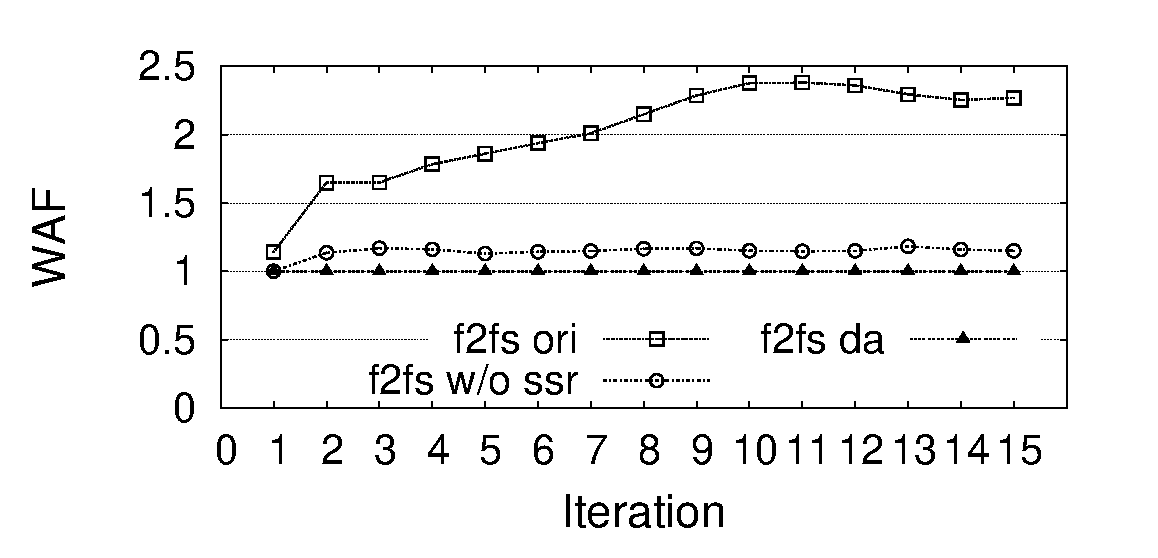
\includegraphics[width=3in]{./comp_gc/170_85_randw_dev}
 \label{fig:170_85_randw_dev}
 }
\subfigure[Total WAF]{
 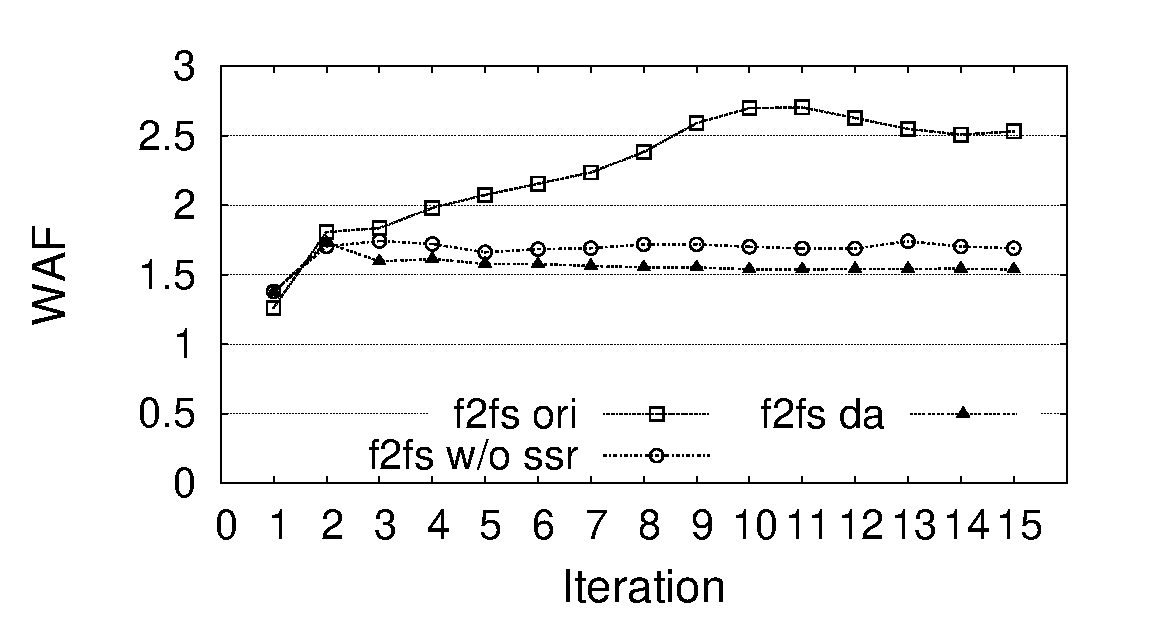
\includegraphics[width=3in]{./comp_gc/170_85_randw_total}
 \label{fig:170_85_randw_total}
 }
 \subfigure[IOPS]{
 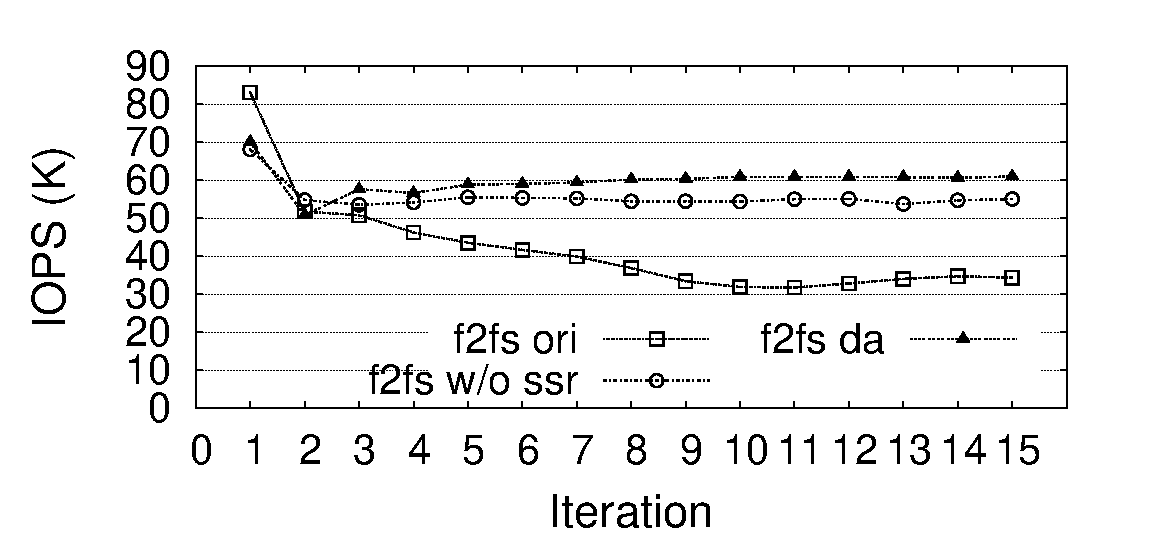
\includegraphics[width=3in]{./comp_gc/170_85_randw_iops}
 \label{fig:170_85_randw_iops}
 }
\caption{The result of Compound Garbage Collection Scenario 1\label{fig:170_85_randw} }
\end{figure*}

Fig \ref{fig:170_85_randw_fs} and Fig \ref{fig:170_85_randw_dev} shows the WAF observed on filesystem and device, respectively. Fig 8(a) shows that using USL increases filesystem WAF by 38\% compared to that of LLS. On the other hand, the WAF of device shown in Fig 8(b) shows that USL is 56\% better than existing F2FS. In the case of LLS, average of 80Gbyte is written using SSR while overwriting 85Gbyte of the created file, which resulted in reducing the WAF in the filesystem. But it forced the device to also perform garbage collection which increased the WAF in storage layer. The overall WAF shown in Fig \ref{fig:170_85_randw_total} shows that as the iterations increase the WAF of base F2FS keeps on increasing. The WAF of USL shows 39.3\% lower than that of LLS.

Fig \ref{fig:170_85_randw} shows IOPS of each configuration. As a result of keeping the overall WAF low, USL achieved about 77.8\% better IOPS than LLS.

\subsection{IO Performance}
\label{subsec:io_performance}

\begin{figure}[h]
\label{fig:benchtest}
\centering

 \subfigure[Sequential Write]{
 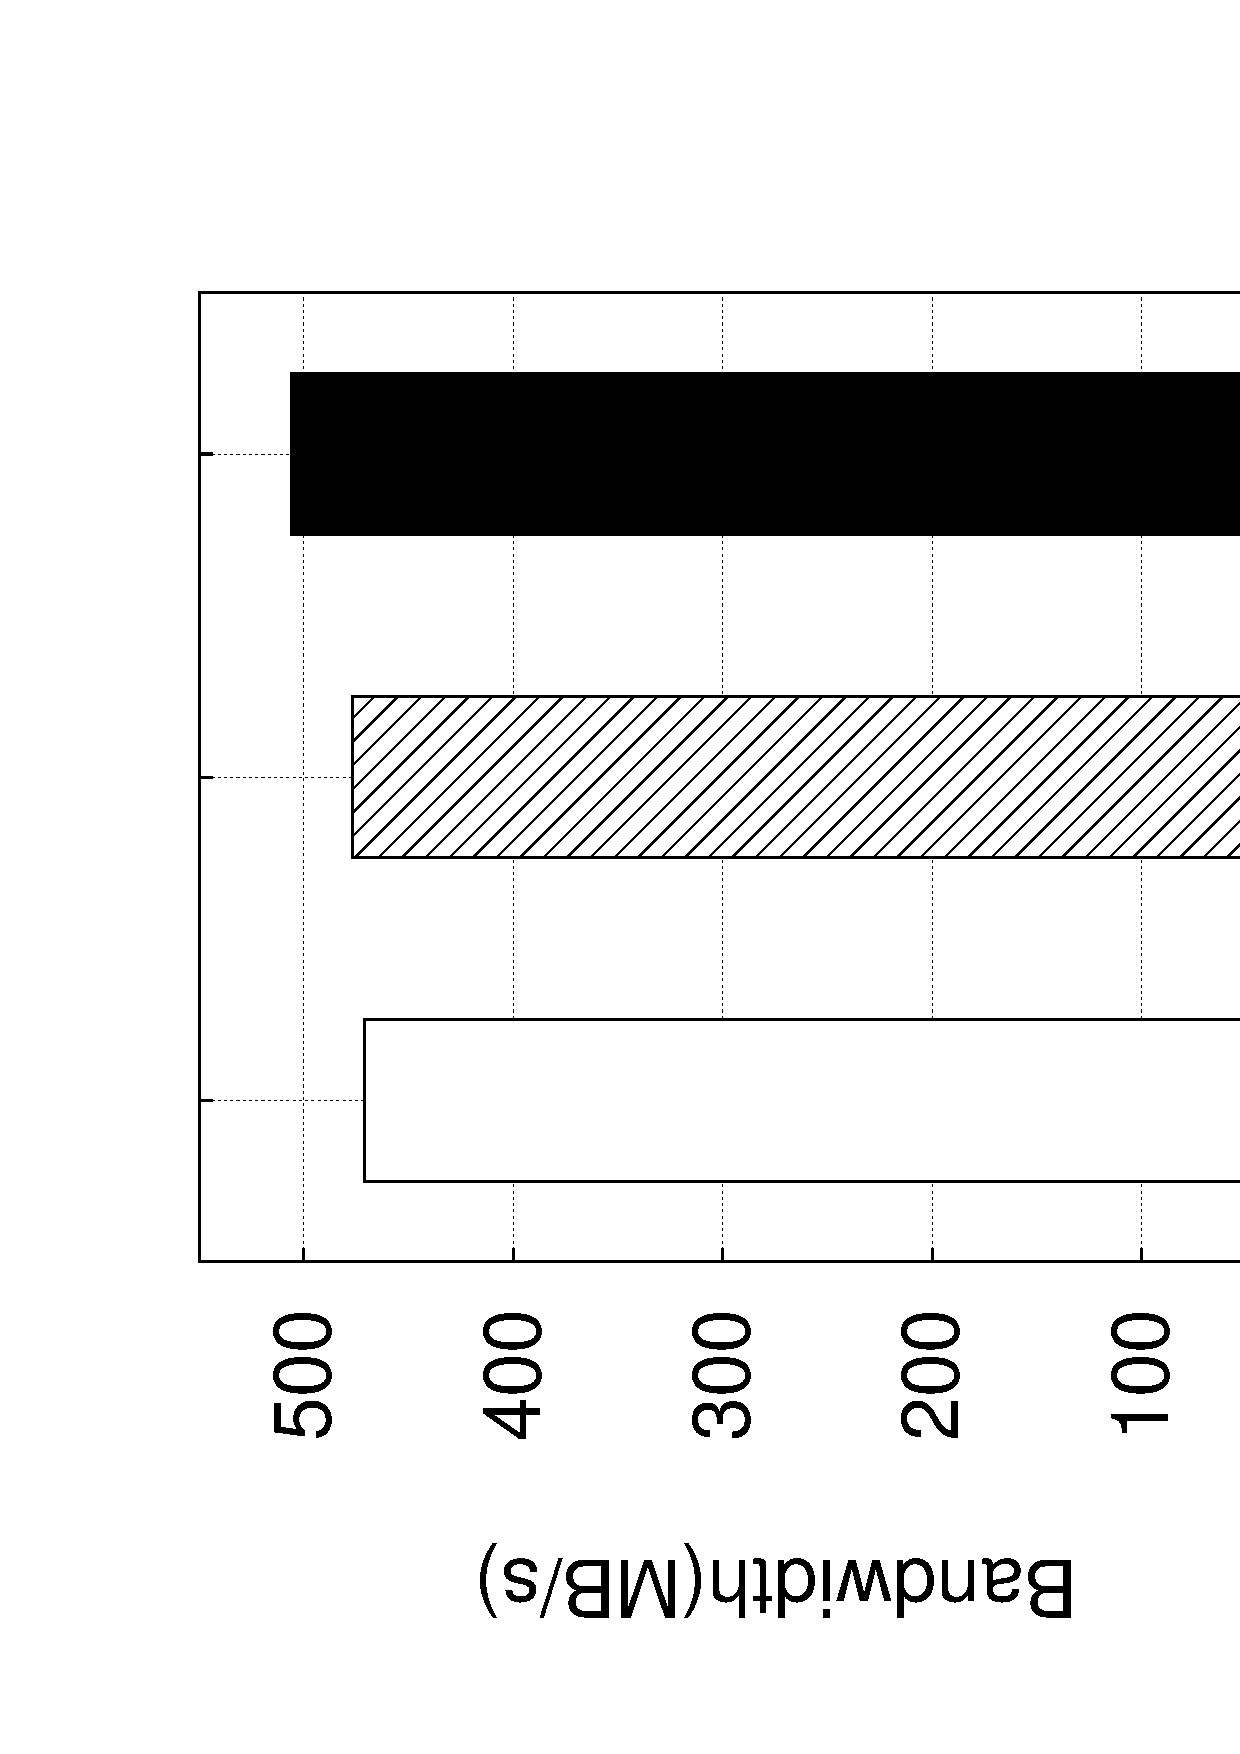
\includegraphics[angle=-90,width=1.47in]{./bench/seq_write}
 \label{fig:benchtest_seqw}
 }
 \subfigure[Random Write]{
 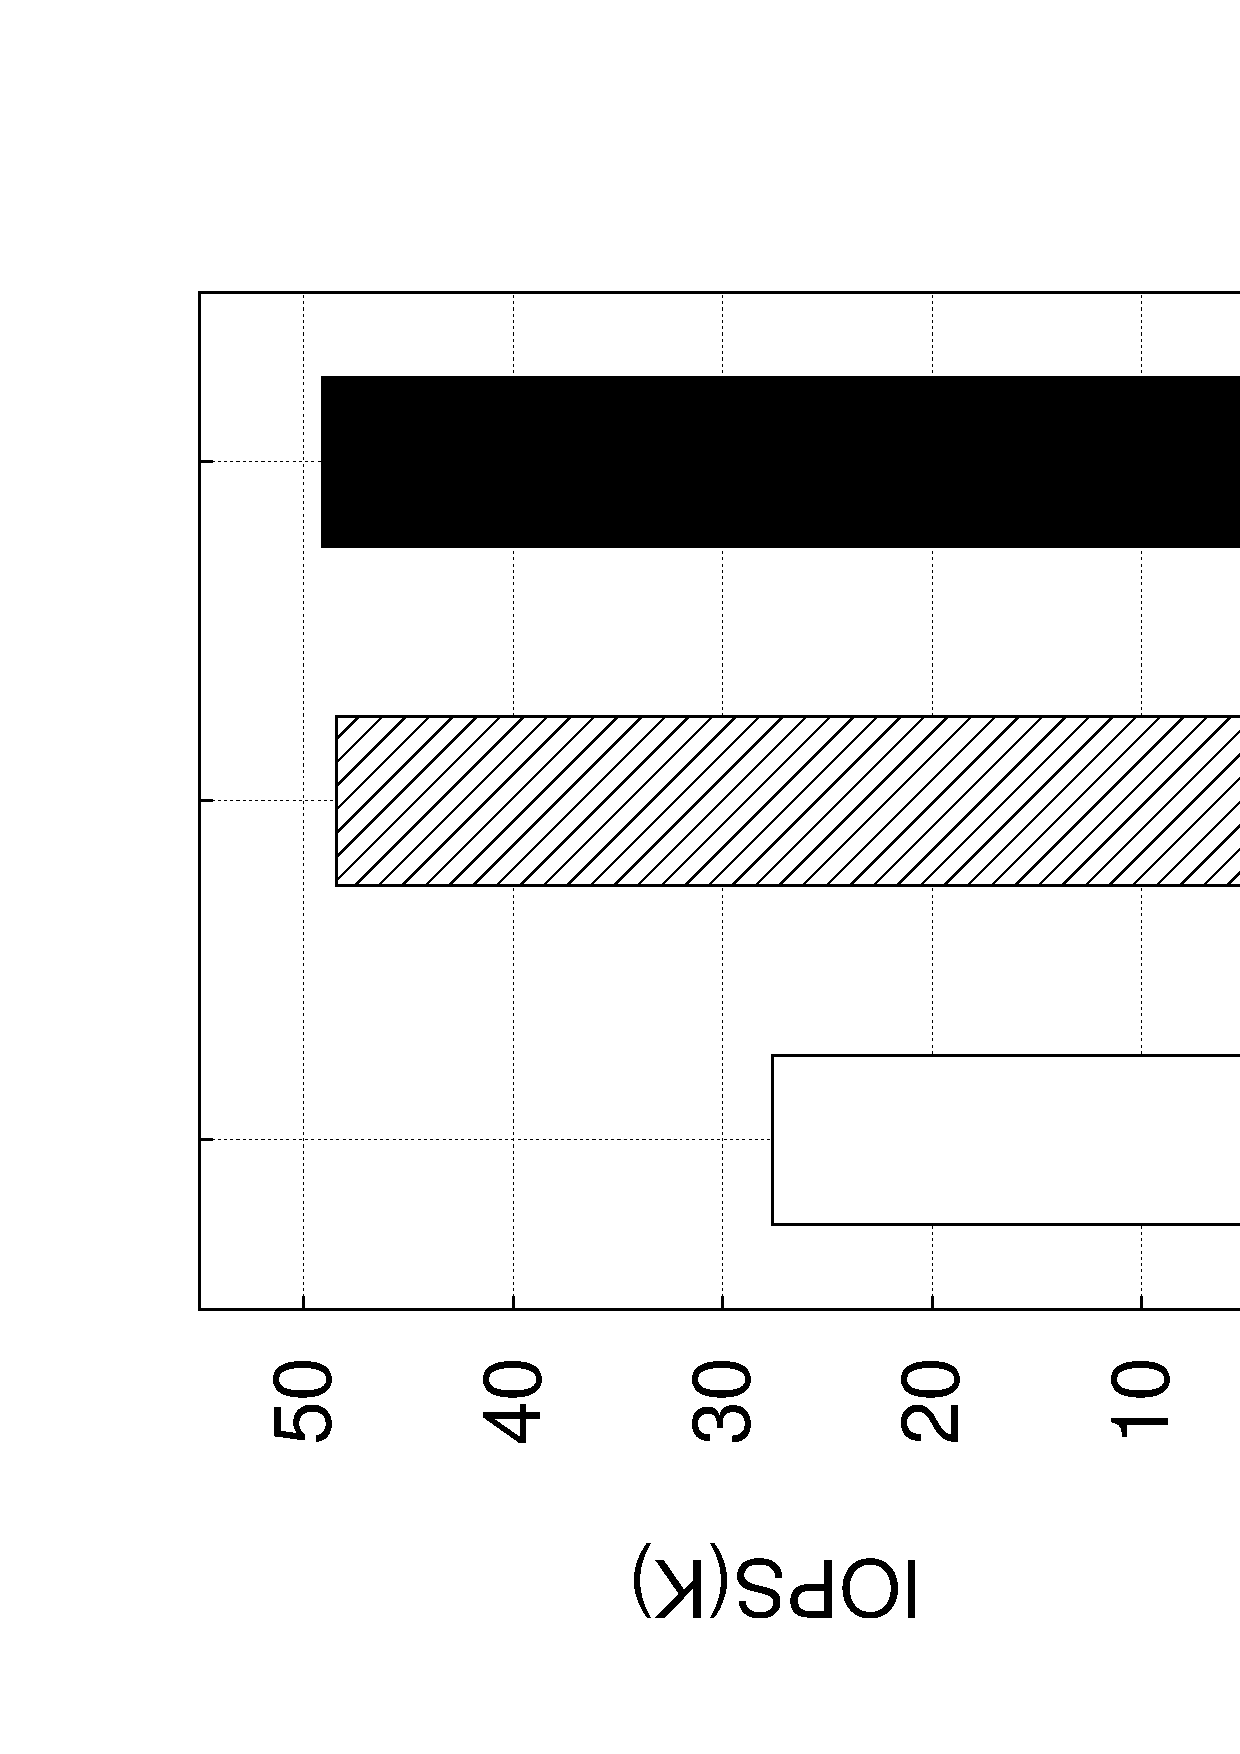
\includegraphics[angle=-90,width=1.47in]{./bench/rand_write}
 \label{fig:benchtest_randw}
 }
\caption{Sequential / Random Write Performance (Sequential Write: 188Gbyte File size, 512Kbyte record size, 2.75Tbyte Total write volume / Random Write: 50Gbyte File size, 8Kbyte record size, 750Gbyte Total write volume)}
\end{figure}

Table \ref{tab:system_info}에 언급된 각 시스템의 Sequential Write과 Random Write의 성능을 측정하여 Fig \ref{fig:benchtest}에 나타내었다. Sequential Write 성능 측정을 위하여 SSD를 각 파일시스템으로 포맷한 뒤, 188Gbyte 크기의 파일 하나를 파티션에 생성하였다. 생성한 파일에 512 Kbyte beffered sequential write을 파일 크기만큼 수행하는 것을 1 iteration이라 하였을 때, 위 결과는 총 15 iteration을 수행하였을 때의 평균 Bandwidth 이다 (Fig \ref{fig:benchtest_seqw}). 실험 결과 LLS의 경우 471Mbyte, INP의 경우 477Mbyte의 Bandwidth를 보여 두 시스템의 sequential write 성능은 큰 차이를 보이지 않았다. 반면 USL의 경우 506Mbyte의 Bandwidth를 보여 다른 시스템 대비 약 6\% 향상된 write 성능을 보였다. 본 워크로드에서 LLS, INP, USL은 각각 1.003, 1.001, 1.003의 WAF가 측정되어 각 로그 계층의 garbage collection overhead는 거의 무시할 수 있다. 그럼에도 불구하고 USL의 성능이 향상된 원인은, LBA를 그대로 PBA로 사용하는 USL의 Main area 매핑 정책으로 FTL 소프트웨어 계층의 불필요한 매핑 변환 overhead를 제거한 결과로 보인다.

LLS와 USL의 성능차이는 Random Write 워크로드에서 더욱 두드러지게 확인할 수 있다. 각 시스템의 Random Write 성능 측정을 위하여 SSD를 각 파일시스템으로 포맷한 뒤, 50Gbyte 크기의 파일 하나를 파티션에 생성하였다. 생성한 파일에 8KByte Buffered random write을 파일 크기만큼 수행하는 것을 1 iteration이라 하였을 때, Fig \ref{fig:benchtest_randw}는 Garbage collection이 동작한 이후 12 iteration의 평균 IOPS를 보여준다. 실험 결과에서 확인할 수 있듯이, INP의 경우 48,447 IOPS, USL의 경우 49,110 IOPS로 근소하게 USL의 성능이 높게 나왔다. 주목해야할 부분은 LLS의 경우 20,212 IOPS로 USL 대비 약 60\% 낮은 성능을 보인다는 점이다. 이는 Section \ref{subsec:case_study_2}에 언급한 Uncoordinated garbage collection의 결과로 보이며, 실제로 Filesystem 계층의 WAF는 1.04로 가비지 컬렉션 overhead가 거의 없으나, Device의 WAF는 2.2로 측정되었다. 이는 이미 파일시스템에서 무효화된 페이지가 디바이스 계층에서 valid page로 남아, 불필요한 valid page copy overhead를 야기함을 확인할 수 있다. 반면 USL의 경우 WAF 값이 1.1이 측정되어, 파일시스템 레벨의 가비지 컬렉션을 통해 uncoordinated garbage collection 문제를 해결하고, 디바이스단의 불필요한 가비지 컬렉션 overhead를 제거함을 확인할 수 있었다.
 
\section{Related Works}
\label{related_works}

Yang et al\cite{yang2014don} illustrated the effect of stacking a log-structured layer on top of another log-structured layer, i.e., using log-structured filesystem on top of SSD. They pointed out that although using log-structured filesystem provides benefit of increased write performance and also provides useful feature such as snapshot, garbage collection on each layer reduces the life of SSD. After log-on-log simulation based on F2FS, they showed that it is better to make keep the size of upper segment larger or equal to the size of lower segment and perform upper layer garbage collection before lower layer garbage collect yields better performance.

Zhang et al\cite{zhangremoving} introduced FSDV(File System De-Virtualizer) to reduce the memory overhead of managing mapping information on both filesystem and storage device. It is a user-level tool that becomes active when either the system becomes idle or system memory is depleted due to increase in mapping information. When FSDB is invoked, it first checks mapping information and makes filesystem to point the physical address and removes logical to physical address mapping information. Their approach reduced the device mapping information to about 75\% at best. However, the worst case scenario forces to store all the logical to physical mapping information. One of the downside of using FSDV is that the memory on the device cannot be smaller than the maximum size of the mapping table.

Josephson et al\cite{josephson2010dfs} introduced Direct File System (DFS) which tries to exploit the maximum performance of NAND Flash Memory. The pointed out that mix of various complex techniques such as block allocation policy, buffer cache, and crash recovery, made filesystem operations too complicated and hinders the performance of underlying storage. They implemented Virtualized Flash Storage Layer (VFSL) in device driver layer which replaces the role of block management and FTL. VFSL keeps mapping information between virtual address and physical address in Flash memory, and also takes care of garbage collection and wear leveling of the device. DFS is a filesystem that exploits VFSL to read and write the flash memory. VFSL is implemented for Fusion IO. The design of DFS is greatly simplified because VFSL manages block allocation and Inode management that used to be manipulated in filesystem. Note that BFSL takes responsible for all the operation. Thus, it does not suffer from compound garbage collection problem. Since VFSL manage virtual to physical address mapping information, it does not have much benefit over the size of mapping table.


\section{Conclusion}

본 논문에서는 중첩된 로그 시스템의 Compound garbage collection 문제를 해결하기 위해 Unified Storage Layer (USL)기법을 제안한다. Unified Storage Layer에서 파일 시스템은 F2FS를 수정하여 사용하며, F2FS 파일시스템과 마찬가지로 파일 시스템 파티션을 메타 데이터를 저장하는 Meta Area와 사용자 데이터를 저장하는 Main Area로 구분한다. USL 기법이 적용된 SSD는 파일시스템의 파티션 정보를 가지고 있으며, 파일시스템의 각 영역에 대해 서로 다른 매핑 방식을 사용하도록 한다. 즉, Random 쓰기 특성을 갖는 Meta Area에 대해서는 페이지 매핑을 사용하였으며, Sequential 쓰기 특성을 갖는 Main Area에 대해서는 LBA를 그대로 PBA로 사용하도록 하여 매핑 테이블을 제거하였다. 이와 같이 각 파일 시스템 영역에 최적화된 매핑 방식을 사용하는 Disaggregate Mapping 기법을 통해 SSD의 메타데이터 크기를 페이지 매핑 방식 대비 54 분의 1로 감소시켰다. 이는 SSD가 메타데이터 관리를 위해 필요한 메모리의 크기를 크게 줄일 수 있음을 의미한다. 더욱이 Main Area에 대해서는 파일시스템에서만 가비지 컬렉션을 수행하고, Main 영역에 할당된 SSD의 플래시 메모리에서는 기존의 가비지 컬렉션 동작을 없애고 Block erase operation만을 수행함으로써, Compound Garbage collection 문제를 해결하였다. USL은 F2FS가 페이지 매핑 방식의 SSD위에서 동작하는 기존 시스템 대비 Write Amplification을 40\% 감소시켰으며, 77\% 높은 IOPS를 보여주어, Layered Log System의 메타 데이터 크기를 크게 감소시킴과 동시에 향상된 입출력 성능을 갖도록 하였다.

\bibliographystyle{acm}
\bibliography{ref}


\end{document}
